\documentclass[12pt]{article}

\usepackage{macros}

\title{Lecture 0 for EE127 (Fall 2018): Optimization Models in Engineering}
\author{Scribes: Nilesh Tripuraneni \textit{(Change This To Your Names)}}
\date{01/01/01 \textit{(Change This to Lecture Date)}}
\begin{document}


\maketitle

\section{Scribing}
\sectionlabel{convexity}

This document provides a scribing template. Try to organize the sections/subsections for your lecture in a coherent way. Also please read the directions detailed in the \emph{instructions.pdf} file contained in the Github (\url{https://github.com/nileshtrip/EE127Notes}).

\subsection{What a scribe should do}
What a scribe should do:
\begin{definition}[Good Scribe]
A good scribe should follow the scribing instructions.
\end{definition}

\section{Convex functions}
We care a lot about convex functions.

\begin{theorem}[The name of the theorem]
\theoremlabel{atheorem}
Although this class is not heavily proof-oriented if the lectures contain any important/useful theorems put them in a theorem environment.
\end{theorem}
\begin{proof}[Proof of \theoremref{atheorem}]
An instructive proof (or reference to a proof in one of the course texts) about convexity might go here.
\end{proof}

\subsection{Examples relating to the aforementioned theorem}
\begin{itemize}
\item You will learn to love linear spaces $\{x\in\R^n\mid Ax=0\}$ and halfspaces $\{x\in\R^n \mid \langle a, x\rangle \ge 0 \}$.
\item You will also encounter the cone of positive semidefinite matrices, denotes, $S^n_+ = \{ A\in\R^{n\times n}\mid A\succeq 0\}$ later in this course. Here we write $A\succeq 0$ to indicate that $x^\trans A x\ge 0$ for all $x\in\R^n.$
\item See \cite{boyd2004convex} for lots of other examples. This is how you should cite a reference. If the reference is not contained in the \emph{notes.bib} file you should add the bibtex (Google Scholar is a good place to get these bibtex blurbs).
\end{itemize}

\begin{fact}
A fun fact about convexity or linear algebra.
\end{fact}

A nice, multi-line equation about convexity,
\begin{align}
& f(1-\gamma)x+\gamma y) \le (1-\gamma)f(x)+\gamma f(y) \\
& f(1-\gamma)x+\gamma y) \le (1-\gamma)f(x)+\gamma f(y)
\end{align}
An in-line equation $f(x) \le f(y)$.

An equation without a label,

\[
f(y) \ge f(x) + g^\trans (y-x)\,.
\]
\begin{figure}[!ht]
\begin{center}
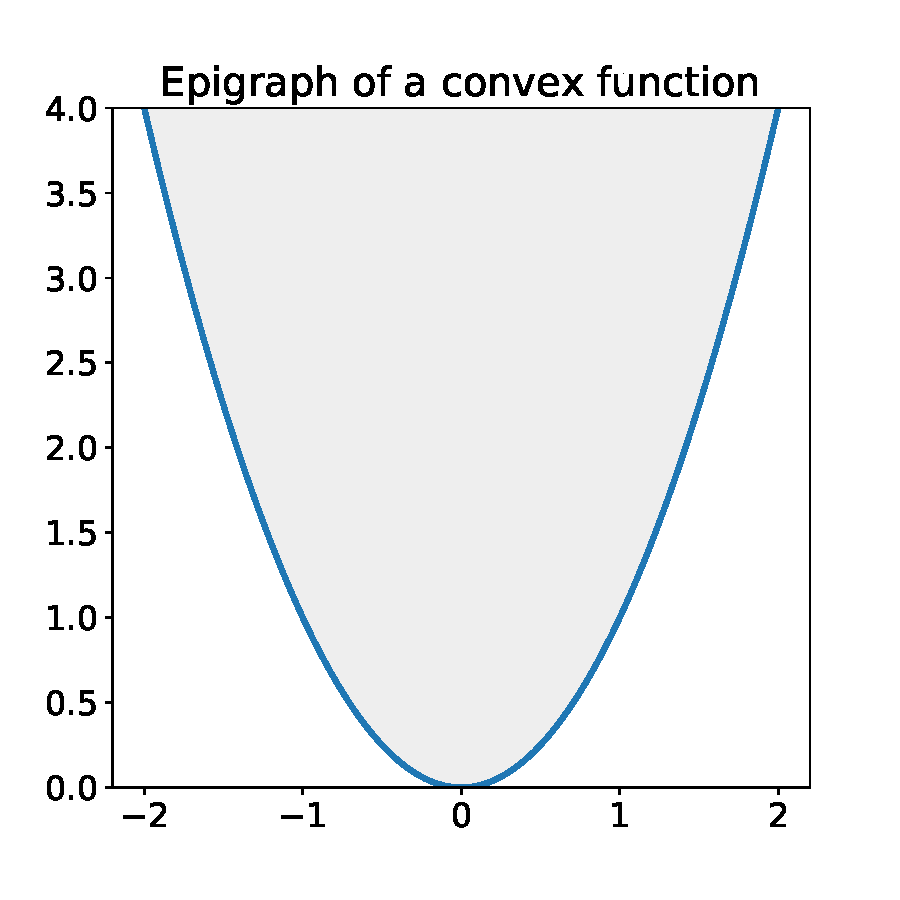
\includegraphics[width=3in]{figures/lecture1-epigraph}
\end{center}
\caption{A fun figure about epigraphs completely unrelated to \propositionref{first-order-taylor}.}
\end{figure}
\subsection{An important characterization perhaps}
\begin{proposition}
\propositionlabel{first-order-taylor}
Something important about differentiability and convexity.
\[
f(y) = f(x)
+ \nabla f(x)^\trans (y-x)
+ \int_0^1 (1-\gamma)\frac{\partial^2 f(x+\gamma(y-x))}{\partial\gamma^2}\rd\gamma
\]
\end{proposition}
\begin{proof}
A nice proof.
\end{proof}


\section{Convex optimization}
We care a lot about ~$f\colon\domain\to\R$ over a convex domain~$\domain:$
\[
\min_{x\in\domain}\quad f(x)
\]

\begin{remark}[Subgradients]
\emph{subgradients} are great!
\[
f(y) \ge f(x) + g^\trans (y-x)\,.
\]
Maybe we need to reference \theoremref{atheorem} here.
\end{remark}

Subgradients are useful for optimizing convex functions.


\bibliographystyle{alpha}
\bibliography{refs}

\end{document}
